\chapter{声明}
本产品不用与任何商业用途,最新版下载地址为:
\href{https://github.com/1411279054/Letax-learning-Note/tree/master/%E5%A4%A7%E5%AD%A6%E7%89%A9%E7%90%86%E5%A4%8D%E4%B9%A0%E6%8C%87%E5%8D%97}{Github}(点击即可下载),不保证题目和答案的正确性(因为本人能力有限),
但如有错误可通过QQ(见图\ref{fig:1}) \footnote{1411279054}或者邮箱\footnote{1411279054@qq.com}联系我。
\begin{figure}[htbp]
	\centering
	
\includegraphics[width=0.3\textheight]{2weima.jpg}
	\caption{二维码}\label{fig:1}
\end{figure}

点击\href{https://github.com/1411279054/Letax-learning-Note/tree/master/%E5%A4%A7%E5%AD%A6%E7%89%A9%E7%90%86%E5%A4%8D%E4%B9%A0%E6%8C%87%E5%8D%97}{Github}后,找到$\mathrm{physics.pdf}$后点击,点击$\mathrm{download}$即可。
\\
\begin{remarkname}
	为什么想到要做这个? 可能是一时兴起吧。其中的习题和解答大部分都是来着老师的课件, 如果你正好用的到的话, 那你就参考参考。有问题随时找我(排版上的错误), 我马上改, 改好最新版的内容我会放在\href{https://github.com/1411279054/Letax-learning-Note/tree/master/%E5%A4%A7%E5%AD%A6%E7%89%A9%E7%90%86%E5%A4%8D%E4%B9%A0%E6%8C%87%E5%8D%97}{Github}上, 现在是期中版本, 应该还会持续更新的, 到时候期末再发出来吧!
\end{remarkname}
\begin{figure}[H]
	\centering
	\parbox[t]{0.3\textwidth}{
		\centering
		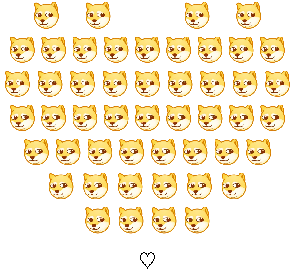
\includegraphics[width=0.29\textwidth]{heart}
	}
	\parbox[t]{0.3\textwidth}{
		\centering
		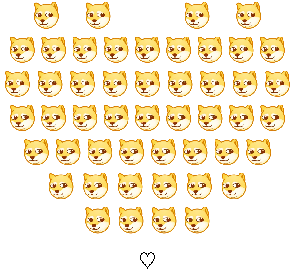
\includegraphics[width=0.29\textwidth]{heart}
	}
	\parbox[t]{0.3\textwidth}{
		\centering
		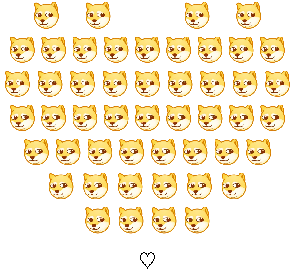
\includegraphics[width=0.29\textwidth]{heart}
	}
\end{figure}